\section{Temporal predictions of rentals}
\label{sec:8_4_regression}

In this section, we describe the task of predicting the number of rentals in the whole city at a given time in the future. Eventually, the same methodology could be applied for each neighborhood. 
This prediction can exploit historical data, i.e., given the time series of rentals in the past, predict the number of rentals in the future. 
If only the past time series are used, the problem falls in the univariate regression class, i.e., the prediction is based only on past data of the same target variable.
Let $x(t)$ be the target variable, i.e., the number of rentals at time $t$.
In the case of prediction with historical data, we predict 
\[
x(t+j)=f(x(t),x(t-1),\ldots, x(t-k)), \, j>0,
\]
as a function $f()$ of the past $k+1$ data points of $x$ itself. $j$ is the horizon of the prediction.

%If we also have other information, we can build a more generic model to consider the dependence to other variables. 
%We want to predict
if other information are present, it possible to predicict a more generic model to consider the dependence to other variables
The goal is to predict
\[
x(t+j)=g(y_1,y_2,\ldots, y_l), \, j>0,
\]
where $\{y_i\}$ are different variables -- possibly other time series themselves (including $x$) -- and $g$ is the model that allows to predict $x$ at time $t+j$.
This problem is a multivariate regression problem, where multiple features are used to predict the target variable $x$.

Considering the time horizon of the prediction, it is possible to formulate two versions of the problem: predict the long-term or short-term usage. In the first case, we build and train a single model using all available data to predict the system usage in the next months.
In the short-term version, we target the prediction of the next time bin $t+1$ only, i.e., $j=1$. In this second case, we build and update a new model at each time bin by adding the latest recorded number of rentals to the training set as soon as it becomes available. 

Both predictions are important for the car sharing provider. For instance, the long-term predictions are important for the company to know if their fleet size is enough to keep up with the expected demand. The short-term is important for the company to know when to take a car down for maintenance, or when and where cars should be eventually relocated to those neighborhoods where the demand is expected to increase shortly. While for long-term prediction we use the time series of the rentals and information about day of the week and hour of the day, for short prediction we can use also the near future weather condition information.  
%\ju{This is NOT TRUE!! WEATHER IS ALWAYS USED!!!}


This work, we consider discrete time, i.e., we split time into fixed size time intervals as defined in the aggregation step -- see Section~\ref{sec:8_3_datasetoverview}. We then build and train several machine learning models to tackle each aforementioned problem. The goal is to compare algorithms in terms of accuracy of the prediction and complexity of the model.
At last, we are also interested in considering models that are interpretable, i.e., that allow us to understand which are the most important features that affect car sharing usage in large cities.
We evaluate all models considering three metrics: APE (absolute percentage error), MAPE (mean absolute percentage error), and RMSE (root mean square error) over the validation set. The APE is defined as
\[
APE=100\sum_{t_i\in V} \frac{\mid x(t_i) - \hat{x}(t_i)\mid}{x(t_i)},
\]
where $V$ is the validation set, $ x(t_i)$ is the actual value of the data at moment $t_i$ and $\hat{x}(t_i)$ is the predicted value. The MAPE is then given by
\[
MAPE=\frac{1}{|V|} \times APE.
\]
And the RMSE is defined as
\[
RMSE = \sqrt{\frac{1}{|V|}\sum_{t_i \in V}{\Big(x(t_i) - \hat{x}(t_i)\Big)^2}}.
\]

\subsection{Prediction models}

We use off-the-shelf machine learning models both for the long-term and short-term scenarios. We evaluate univariate models: a simple baseline (BL) approach, the autoregressive moving average (ARIMA) and the seasonal autoregressive moving average (SARIMA) algorithms. 
Univariate models do not account for the influence of other time-variant factors such as weather conditions, time of day, number of emergency calls, etc. 
To account for that, we also investigate the performance of linear regression, random forests Regression (RFR), Support Vector Regression (SVR), and long-term short-term memory neural networks (NN).

We add categorical features (the day of the week and weather, for instance) to these algorithms in order to improve on the univariate models. Following correct practices~\citep{jain1990art}, we represent each categorical feature as many binary variables, one for each category. For example, when representing a given weather type, the corresponding binary variable will be set to $True$ while all the other weather-related variables to $False$.
We used the algorithms implementation in Python libraries \texttt{scikit-learn}\footnote{\url{https://scikit-learn.org/}}~\citep{scikitlearn} and Keras\footnote{\url{https://keras.io/}}. 
%The code for the analysis is publicly available\footnote{\url{https://github.com/dougct/carsharing-prediction}}. 
For details about each model, we refer the reader to~\citep{Bishop:2006}. 
%\dt{
In this implementations, we started with the library's default hyperparameters and conducted a grid search in order to find a set of such parameters that worked well with the described models. We report the range of the grid search along with the description of the models below.
%}


\textbf{Baseline.} A simple approach to determine $x(t+j)$ in a time bin is to take the average number of rentals in the same time bins in the available past days. 
We compare all the prediction models to this baseline. 

\textbf{ARIMA.} ARIMA (autoregressive integrated moving average) is widely used to predict time series data.  ARIMA models are a combination of autoregressive models with moving average models. The creation of an ARIMA model involves specifying three parameters $(p, d, q)$. The $d$ parameter measures how many times we have to differentiate the data to obtain stationary data. After determining $d$, we use sample partial auto correlation function to get the value $p$. Finally, we determine the order $q$ by looking at the sample auto correlation function of the differentiated data. 
For simplicity, we restricted the grid search to find the best parameters values to the range $[0, 3]$. The combination that gave the best results is $(p, d, q) = (2, 0, 1)$.


\textbf{SARIMA.} A SARIMA model incorporates the seasonality (periodicity) of the data into an ARIMA model, enhancing its predictive power. For instance, when modeling a time series, it is often the case that the data has a daily, weekly, or monthly periodicity. We used previous ARIMA model with an additional explicit daily seasonal component ($p=7$ as the number of time bins in a day in this case). 

\textbf{Linear Regression.} We fit a linear model, by finding the coefficients that multiply each feature. 

\textbf{SVR.}  In the experiments, we use a Support Vector Regression (SVR) model with the following combination of parameters, which produced the best results among the values we tested: $C = 1000$, $\gamma = 0.1$, and $\epsilon = 0.1$, with the RBF kernel. 
%\dt{
The values for the parameters $\gamma = 0.1$, and $\epsilon = 0.1$ were evaluated in the range $[0, 1]$, and for the $C$ parameter we considered the range $[1, 10000]$, using exponential steps. The value 1000 was chosen once it provided a reasonable balance between model performance and generality.
%}

\textbf{RFR.} Random Forest Regression is an ensemble learning method that can be used  for regression. The decision is based on the outcome of many decision trees, each of which is built with a random subset of the features. One advantage of random forests over linear regression is that the forest model is able to capture the non-linearity. Another advantage of RFR is that they are interpretable models, i.e. they offer a ranking of the most important features for the prediction problem. Here, we use 50 decision trees\footnote{Here, interpretable refers to the fact that it is possible to understand the decision taken by the classification model. However, interpretability has not to be confused with explainability, which refers to the motivations of the decision. The latter is only possibly via domain knowledge.}. 
%\dt{
In this model, we used the default library parameters, but we evaluated it with different numbers of trees, for which the results are shown in the next sections.
%}

\textbf{Neural Networks.} We also consider a  Long Short-Term Memory (LSTM) Neural Network  model. LSTMs have a memory that helps capturing past trends in the data, which may favor the prediction task. We experimented with several different architectures. The best results were obtained with a three layer architecture where the input layer has 64 neurons (one for each feature), the dense layer has 4 neurons, and the output layer has one neuron. %\dt{
We tested different configurations for the architecture: the number of neurons was varied in the range $[4, 128]$ for the first layer, and in the range $[4, 32]$ for the second layer. Because of the nature of the task (regression and not classification), the number of neurons in the third layer was set to one.
%}
In the experiments, to balance prediction accuracy and training time, the model was trained for 50 epochs. As we will see, increasing the number of epochs to more than 50 has no significant effect (less than 1\% reduction in the MAPE, on average) on the performance of the model.



\subsection{Long-term predictions -  Results}

Here we predict the FFCS demand for cars in the future months given a model built on the previous months. We use in the experiments the nine months of 2017 of car sharing usage of Vancouver. 
Given the volume of rentals in the training period, we try to predict the number of rentals in the validation period. For that, we use a  model that is trained once and then used to perform all the predictions in the validation period. 
The training set consists in the volume of rentals for the first six months, and the validation data consists of volume of rentals for the next three months.

Table~\ref{tab:8_4_results-stationary-models} shows the average mean absolute percentage error (MAPE), the standard deviation of the APE, and the RMSE for each of the prediction models.
%\ana{it is missing to cite the other measures.} 
The models that rely only on the time series (ARIMA and SARIMA) are able to capture some patterns in the data, as their performance is considerably better than the baseline. However, the multivariate models perform better, with Random Forest Regression reaching the best performances. In figure~\ref{fig:random-forests-stationary} we show the comparison between the actual values and the prediction in one month of the validation set using the Random Forest Regression model (orange dashed line). Overall the model is able to predict quite well the daily and weekly periodicity of rentals, but in general slightly underestimates the actual number of rentals. This could be due to the fact the training period refers to the first six months of the year, during which the average number of rentals is lower than during the validation period in fall.



\begin{table}
 \centering
  \begin{tabular}{ccccl}
  \toprule
    \textbf{Prediction Model} & \textbf{MAPE [\%]} & \textbf{$\sigma$(APE) [\%]} & \textbf{RMSE}\\
    %\textbf{Model} & \textbf{} & \textbf{Standard Deviation} & \textbf{}\\
    \midrule
    Baseline                   &  40.05 &  44.95 & 321.32 \\
    ARIMA                      &  25.53 &  19.68 & 238.87 \\
    SARIMA                     &  21.15 &  21.74 & 159.17 \\
    Linear Regression          &  15.80 &  15.61 & 178.57 \\
    Support Vector Regression  &  15.12 &  16.14 & 179.99 \\
    Random Forest Regression   &  14.63 &  11.62 & 157.40 \\
    Neural Networks            &  15.83 &  16.60 & 187.08 \\
  \bottomrule
\end{tabular}
\caption{Long-term temporal prediction - Mean Absolute Percentage Error (MAPE), Standard Deviation of the Absolute Percentage Error (APE) and Root Mean Square Error (RMSE) for each prediction model in the validation set.}
\label{tab:8_4_results-stationary-models}
\end{table}

\begin{figure}
    \begin{center}
            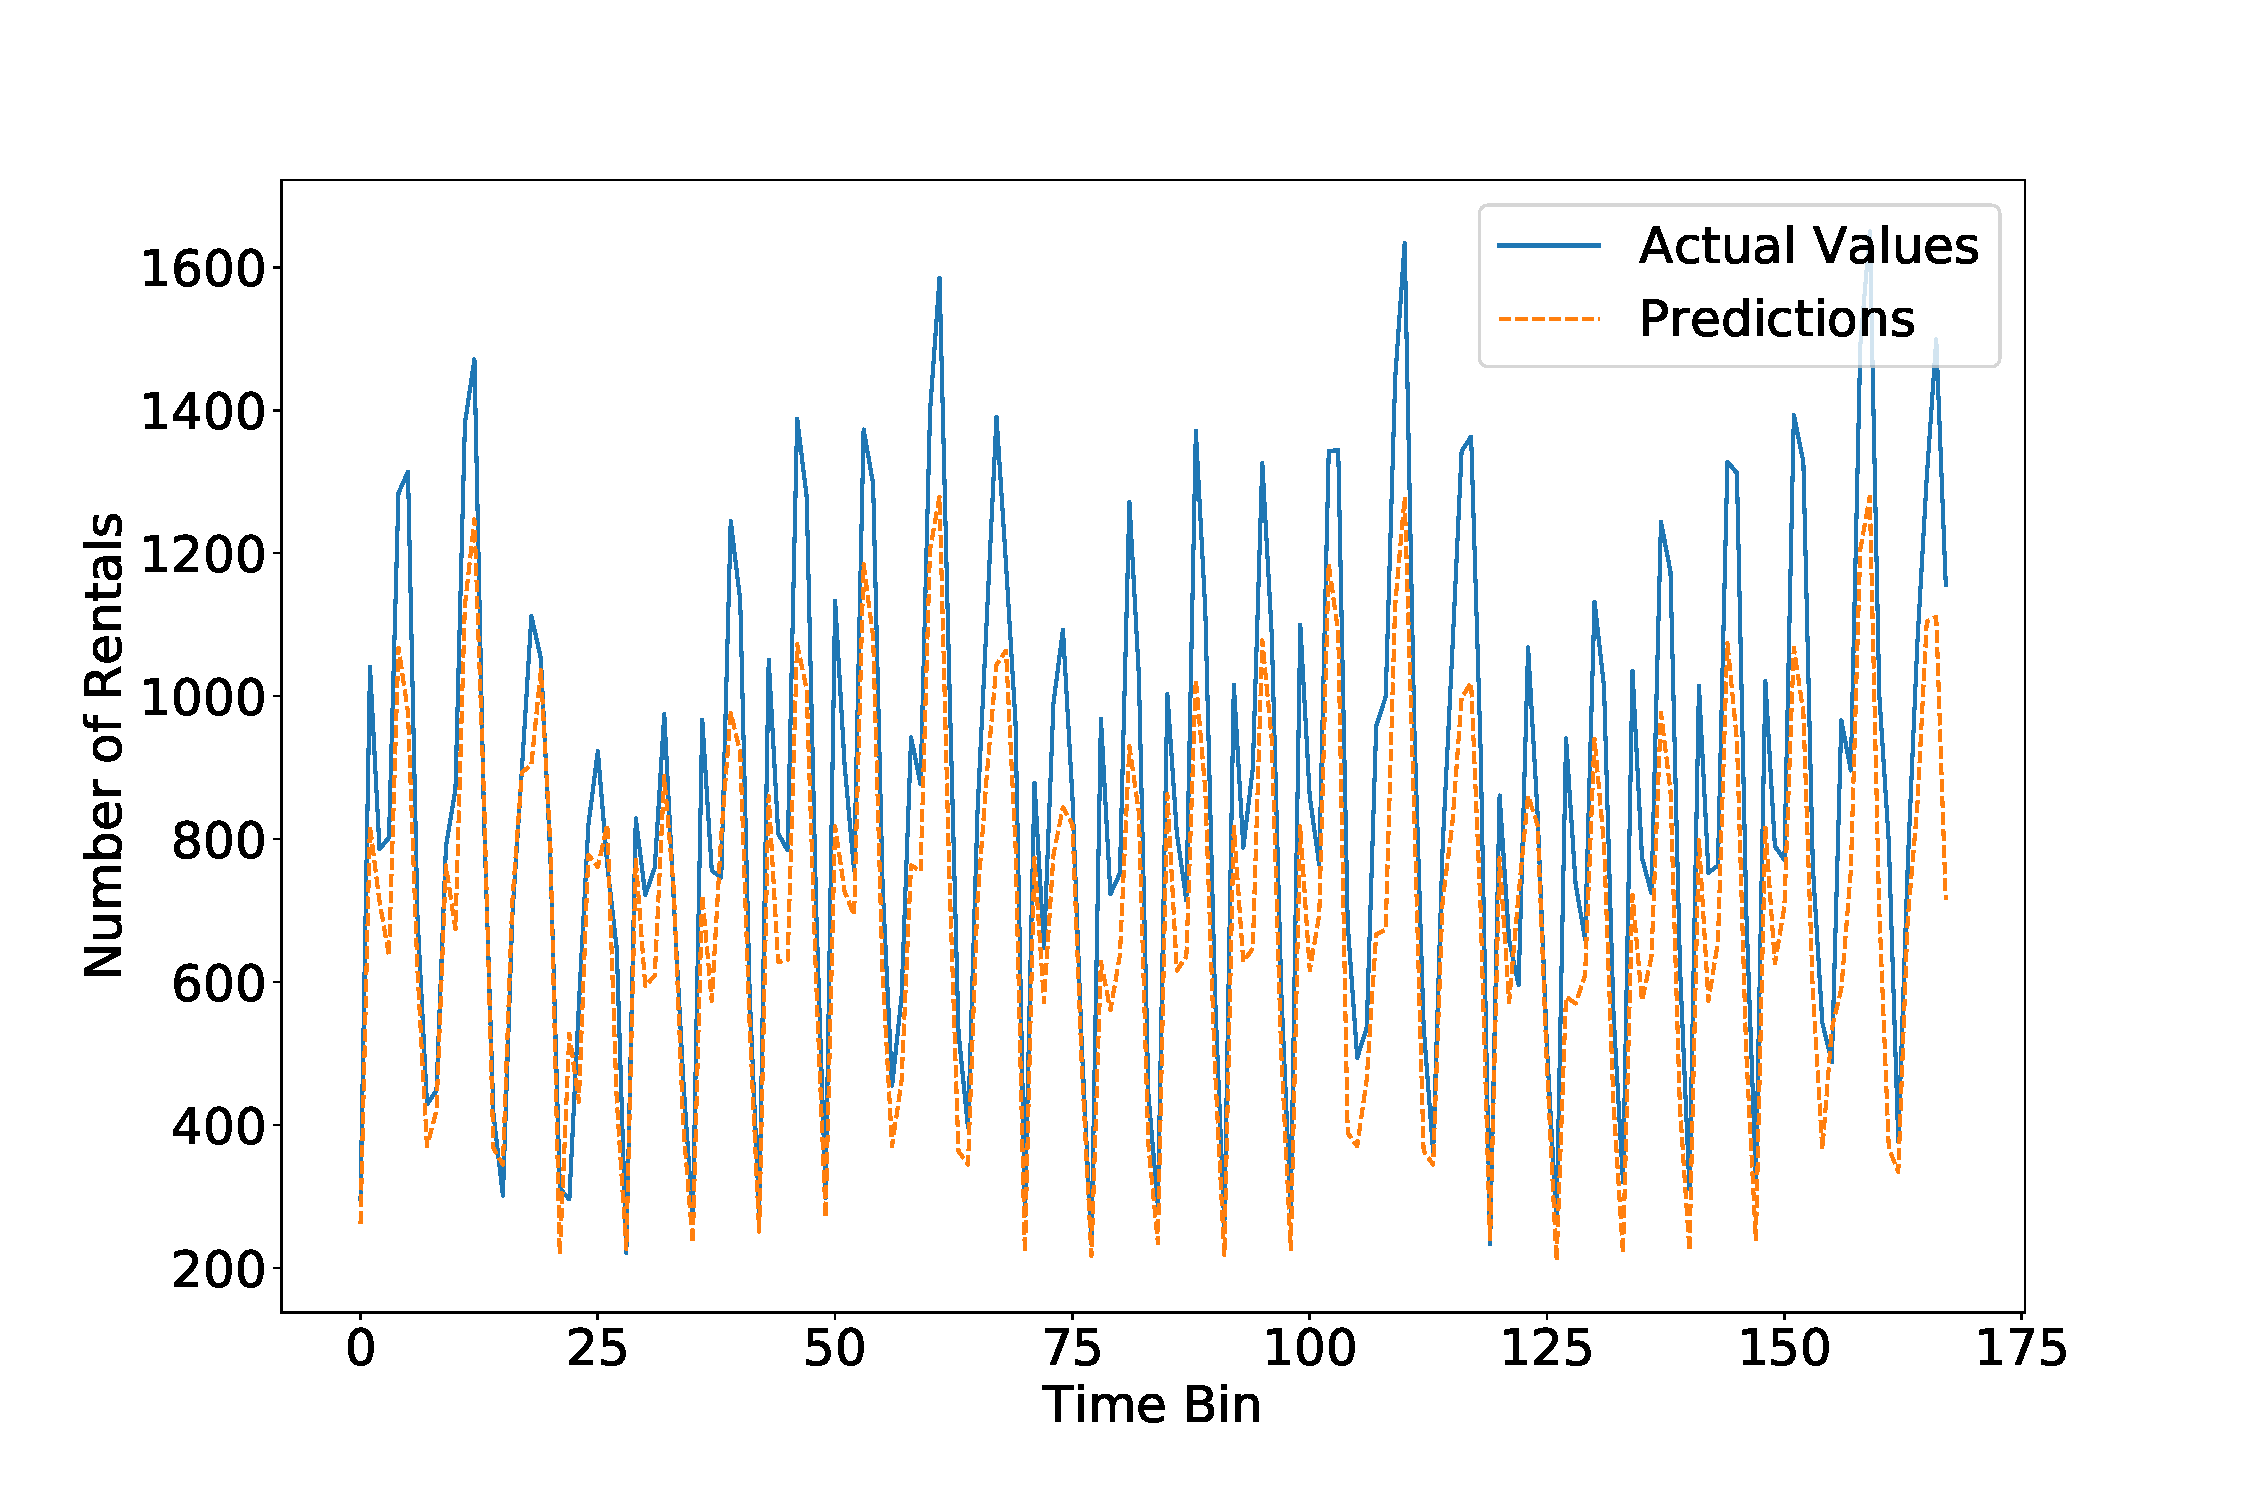
\includegraphics[width=0.65\columnwidth]{figures/temporal_analyses/RandomForestStationaryPredictions.pdf}
        \caption{Long-term temporal prediction - Performance of the RFR model in one month of the validation set. The difference in the total number of time bins and the actual number of hours in the month are due to missing data (crawler failures).}
        \label{fig:8_4_random-forests-stationary}
    \end{center}
\end{figure}

%\ju{CHECK MAPE AVERAGE in ALL TABLES -> it does not make sense. It is either MAPE ou APE Average}.

\subsection{Short-term predictions -  Results}

We now tackle the problem of predicting the demand of cars in a city in the next time bin. 
Differently from the long-term predictions we use adaptive models, hence the model is re-trained every time new data is made available, so then we can add it to the training set.
We here focus on the following prediction task: given the volume of rentals per time bin period for a specific number of past days and the weather conditions, predict the number of rentals in the next time bin period.

We study this prediction task using two approaches: expanding window and sliding window. 
In the \emph{expanding window} approach, after making the first prediction, we add the actual value to the training set, therefore increasing the amount of data available for training in the next step. 
To train the models, we first set aside 24 days of data for validation, and start with 28 days of training data. 
In the \emph{sliding window} approach, after making the prediction we remove the oldest training data and add the actual value to the training set. Therefore, the training set size is always the same during the evaluation of the models. To train the models, we consider different sliding windows sizes (from 7 to 28 days), and validate on the same validation set of 24 days as with the expanding window. 

\begin{table*}
\centering
\begin{tabular}{@{}rrrrcrrrr@{}}
\toprule
& \multicolumn{3}{c}{Expanding Window (starting: 28 days)} & \phantom{abc} & \multicolumn{3}{c}{Sliding Window (28 days)} \\
\cmidrule{2-4} \cmidrule{6-8}
 {Prediction Model} & \textbf{MAPE [\%]} & \textbf{$\sigma$(APE) [\%]} & \textbf{RMSE} && \textbf{MAPE [\%]} & \textbf{$\sigma$(APE) [\%]} & \textbf{RMSE} \\ 
 %& \textbf{Average} & \textbf{Std.  Dev.} & \textbf{Average} && \textbf{Average} & \textbf{Std. Dev.} & \textbf{Average} \\ 
 \midrule
  \textbf{Baseline}                     & 20.12 & 16.64 & 195.53 && 20.12 & 16.64 & 195.53 \\
  \textbf{ARIMA}                        & 36.01 & 35.87 & 306.80 && 36.52 & 36.60 & 305.50 \\
  \textbf{SARIMA}                       & 17.60 & 20.01 & 160.42 && 18.02 & 21.75 & 163.94 \\
  \textbf{Linear Regression}            & 18.28 & 20.38 & 179.11 && 18.11 & 20.55 & 178.61 \\
  \textbf{Support Vector Regression}    & 12.22 & 15.62 & 128.72 && 12.87 & 18.52 & 136.14 \\  
  \textbf{Random Forests Regression}    & 9.71  & 8.34  & 104.99 && 10.08 & 12.23 & 109.47 \\
  \textbf{Neural Networks}              & 10.52 & 12.93 & 128.84 && 10.52 & 12.74 & 123.55 \\
\bottomrule
\end{tabular}
\caption{Short-term temporal prediction - Mean Absolute Percentage Error (MAPE), Absolute Percentage Error (APE), and Root Mean Squared Error (RMSE), for each prediction model in the validation set.}
\label{tab:8_4_results-dynamic-models}
\end{table*}

\begin{figure}
    \begin{center}
            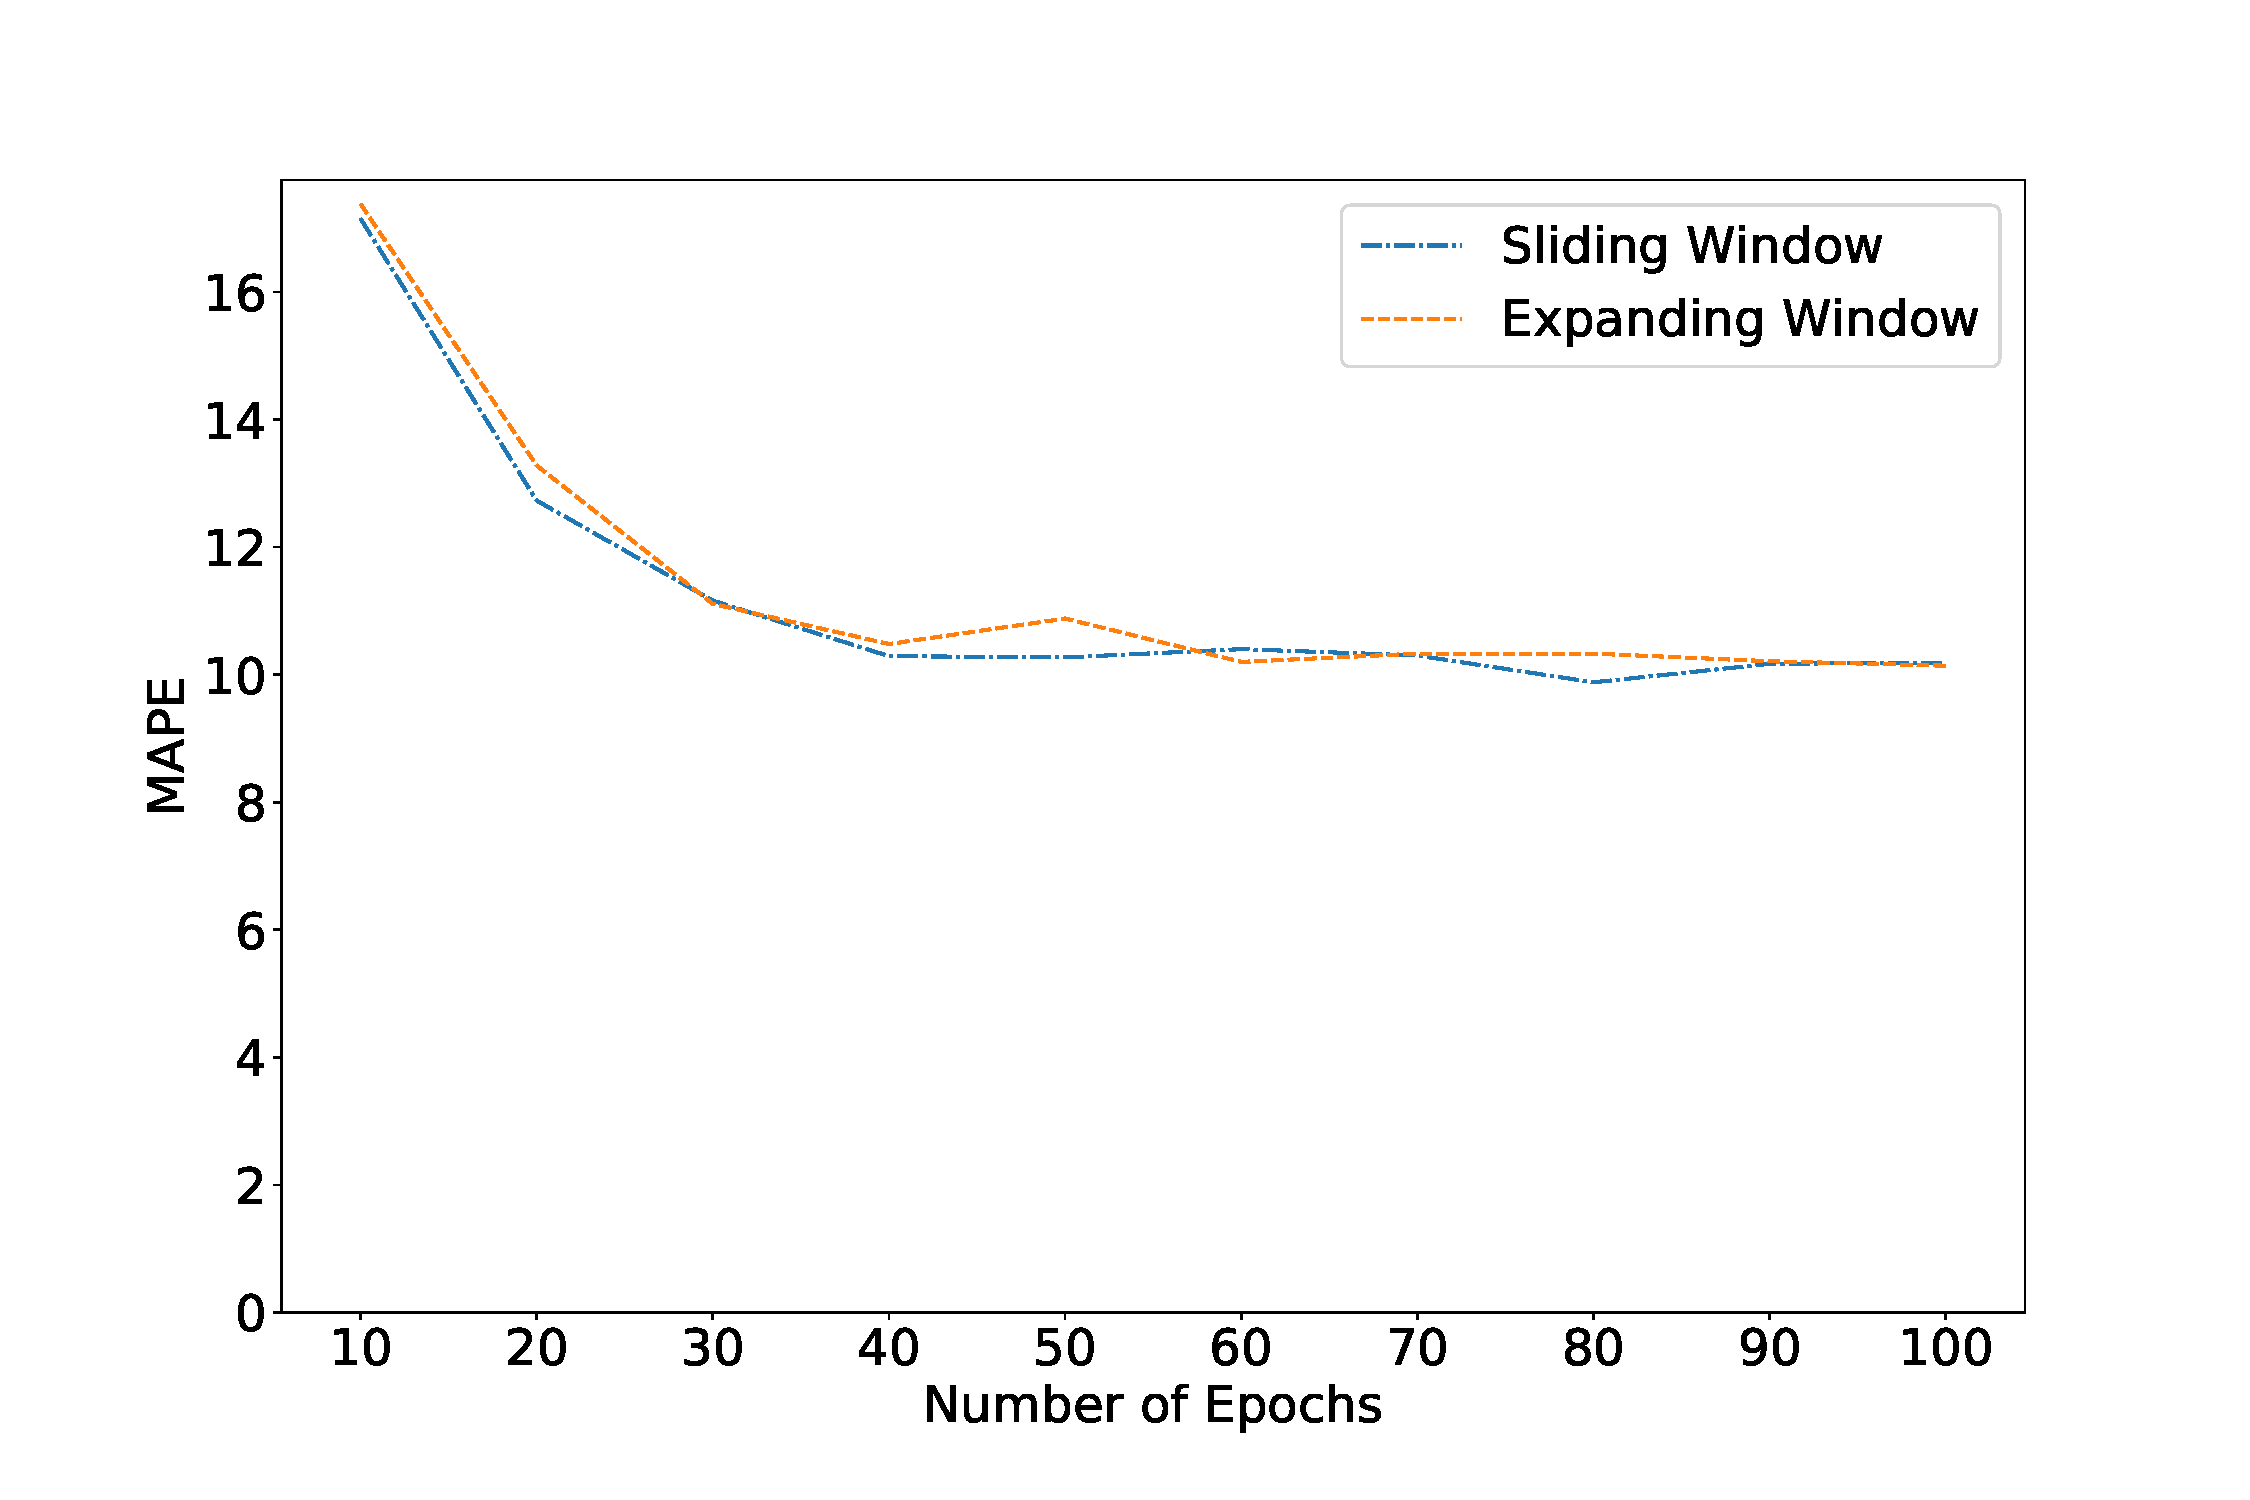
\includegraphics[width=0.65\columnwidth]{figures/temporal_analyses/MAPEEpochs.pdf}
        \caption{Effect of the number of epochs on the performance (MAPE) of the Neural Networks model.}
            \label{fig:8_4_epochs-mape}
    \end{center}
\end{figure}

\begin{figure}
    \begin{center}
            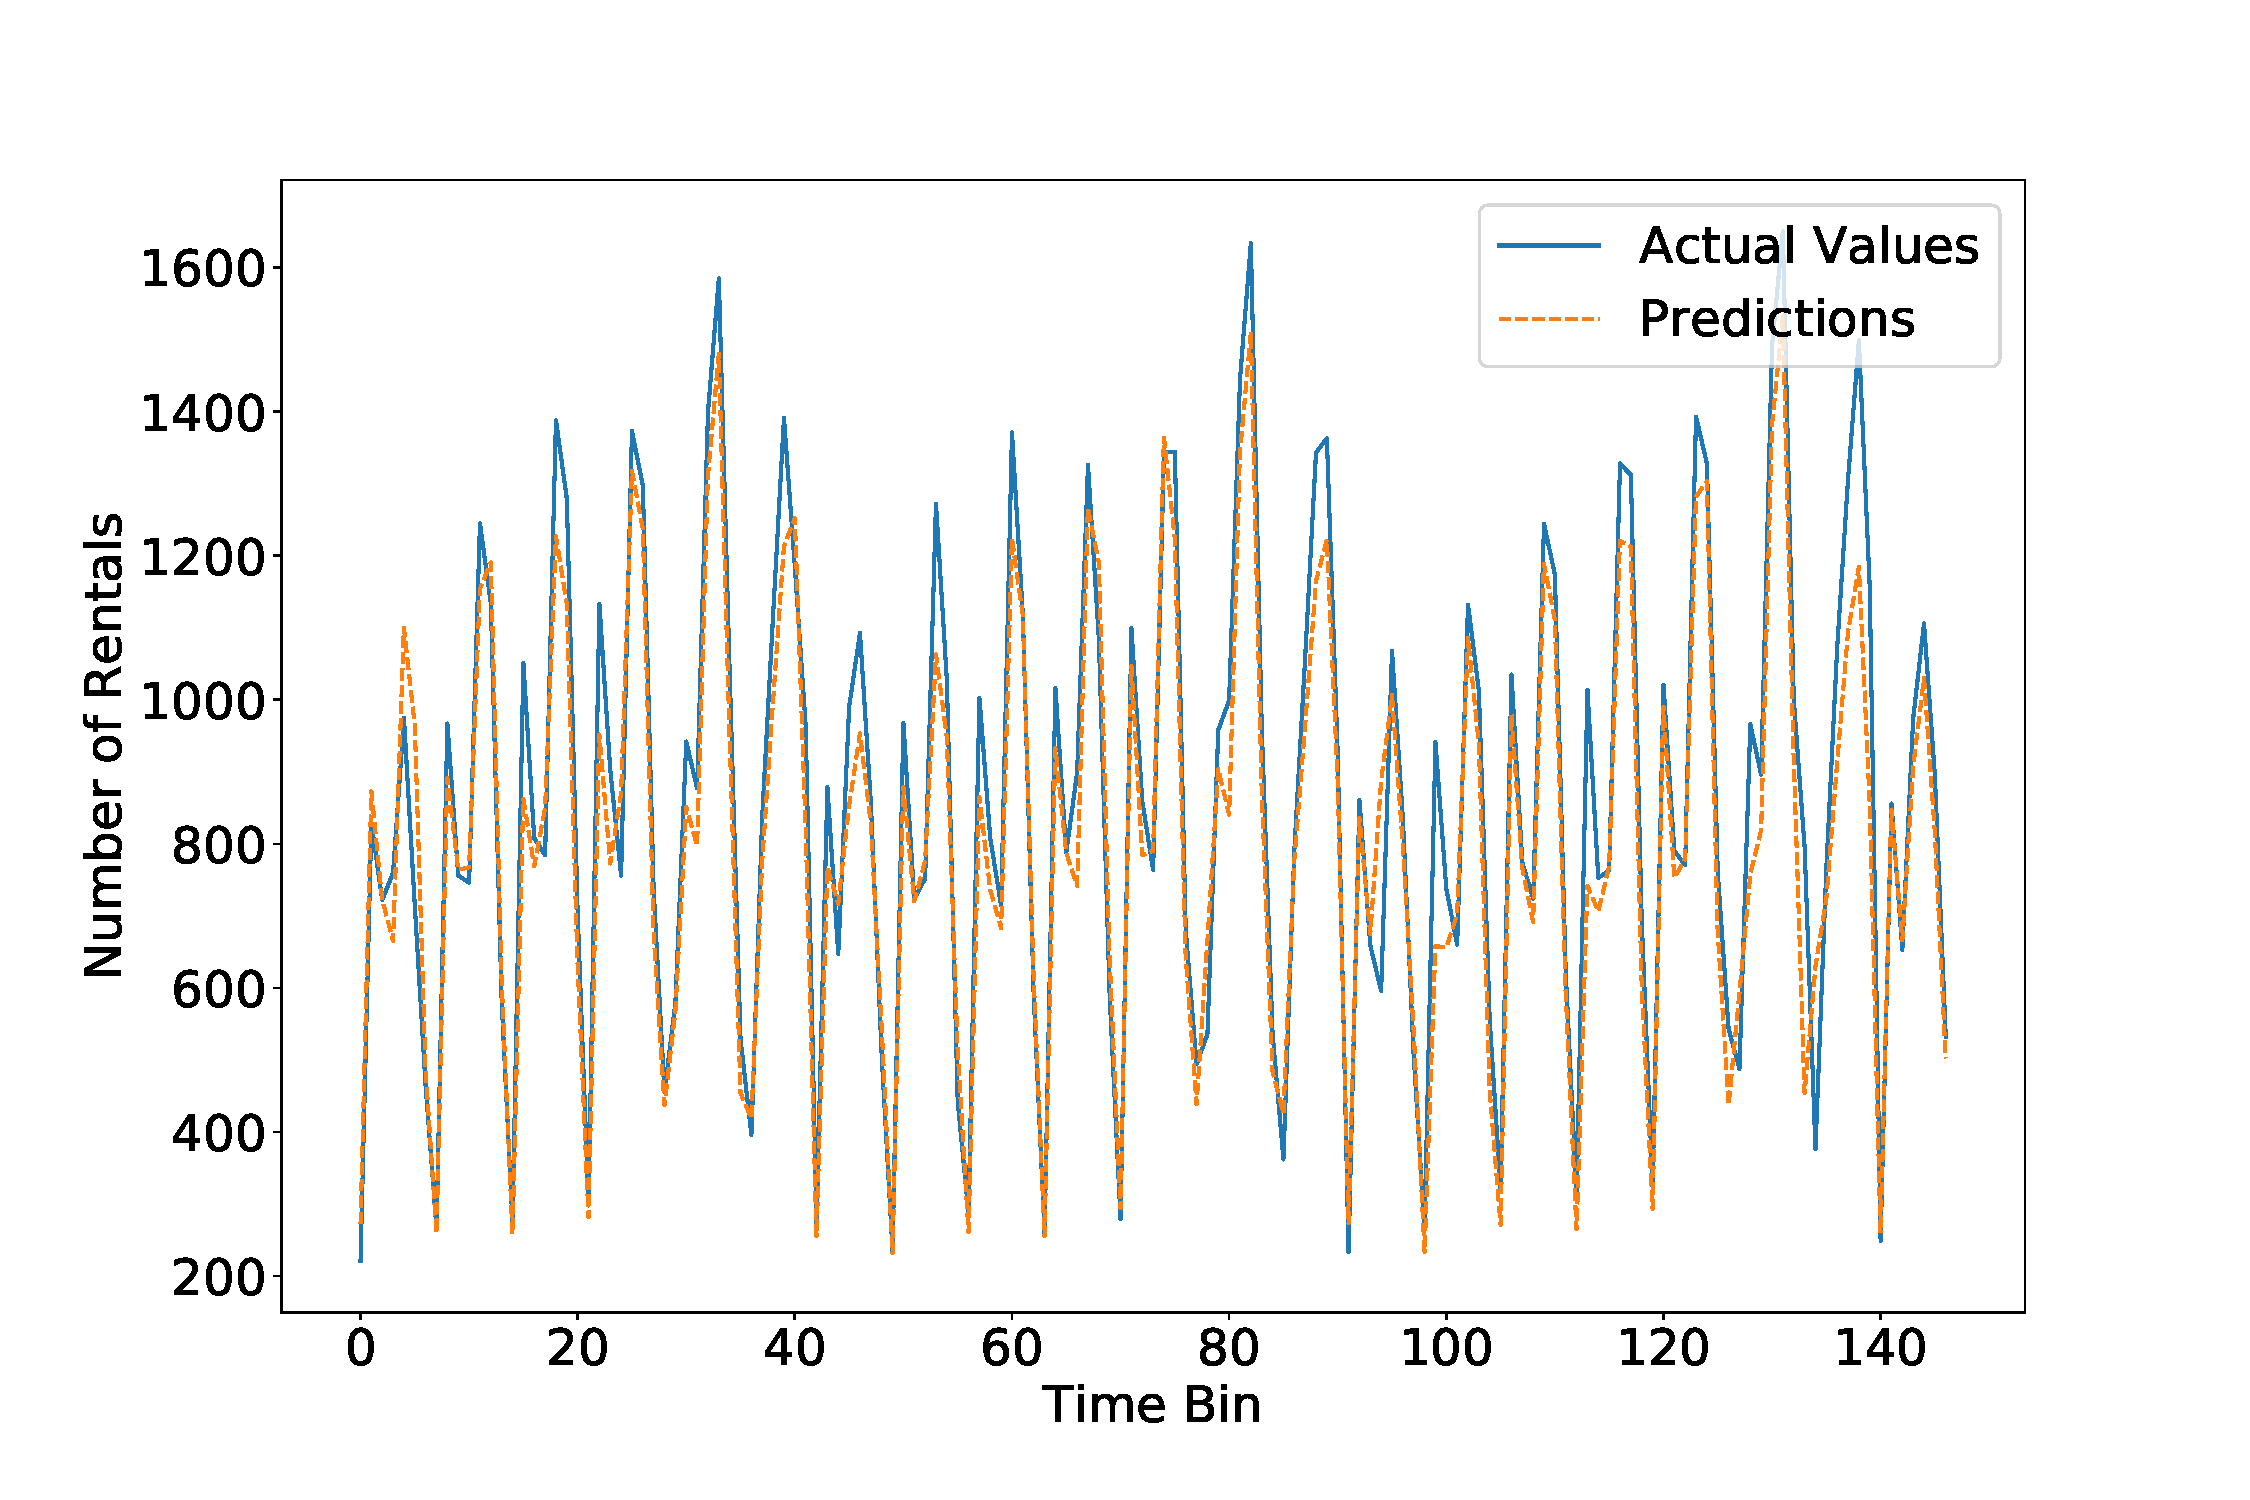
\includegraphics[width=0.65\columnwidth]{figures/temporal_analyses/RandomForestExpandingPredictions.pdf}
        \caption{Short-term temporal prediction - Performance of the RFR model with expanding window in the validation set (24 days).}
            \label{fig:8_4_random-forests-dynamic}

    \end{center}
\end{figure}


In Table~\ref{tab:8_4_results-dynamic-models}, we compare the performance of all models using the two approaches. The best results for the sliding window approach were obtained with the largest possible window (28 days). The expanding window approach offers slightly better results, which can be attributed to the fact that the model can exploit more data and the patterns are not changing rapidly in time. Again, the multivariate models, and in particular the Random Forest Regression model, reach the best performance. Interestingly, the Neural Network model performs similarly to other models, suggesting that, for this specific use case, a simple and more interpretable model like a RFR is enough.
Furthermore, as shown in figure~\ref{fig:8_4_epochs-mape}, increasing the number of epochs does not have a significant effect on the performance of the Neural Networks model.

We show in figure~\ref{fig:8_4_random-forests-dynamic} the performance of the best model, i.e., RFR with expanding window. In this short-term formulation of the problem the prediction naturally adapts to changes over time, obtaining better predictions with respect to long-term prediction. Moreover, the weather data also provides useful information. 



We now explore the importance of each feature for the model by analyzing the RFR feature ranking.  
When training a tree, it is possible to compute how much each feature decreases the tree's weighted impurity. For a forest, the reduction in impurity from each feature can be averaged and the features can be ranked according to this measure. This gives a simple and interpretable feedback on which features are most useful for the prediction. 
We find that the most important features for the model are: (i) if we are in the daily peaks from 3\,pm to 9\,pm, (ii) during the night (0\,am - 6\,am) or (iii) if we are on a Friday and Saturday. Interestingly, the most important weather condition for the regressors is the presence of clouds, while the second one is a (rare) condition of presence of fog, mist and rain in the considered time bin. 

% Discussion about the effect of weather.
%\dt{
\subsection{The effect of weather information}

At this point, it is relevant to discuss the importance of weather forecast for the predictions.
First, for the long-term predictions, we did not use any weather information, as that would require perfect weather forecast in a period far in the future (in this case, three months). In order to validate the effect of weather in this idealized situation, we assumed such perfect forecast and evaluated the models using weather information as a feature. By assuming perfect forecast, we are able to set an upper bound on the effect of weather information on the models. The results show that, on average, weather information improved the models by about 3\% on average.

Second, for the short-term predictions, we can use weather information. We assume perfect weather forecast in the short-term (next three hours). This assumption is reasonable once weather forecast for such short periods should be quite close to perfect. By doing so, we filter out any dependence on the particular weather forecast technique used (which could vary across different places/countries and is therefore out of the scope of this work). 

According to the feature importance, among the features used for the short-term predictions (day of the week, hour of the day, and weather type), the weather is the least important feature. As such, we do not expect a great impact of weather mispredictions on the results. Indeed, the results with the random forests model (the one with the best performance among the models we evaluated) show that by removing weather information from the features the prediction accuracy decreases  by less than 2\% on the MAPE.
%}